\begin{figure}[h!]
	\centering
	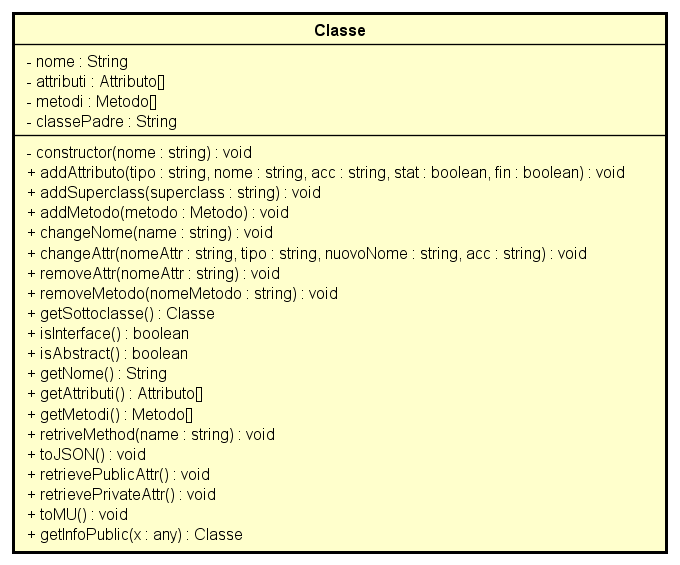
\includegraphics[scale=0.8]{res/sections/SpecificaFrontEnd/Services/Disegnetti/classe.png}
	\caption{Diagramma della classe Classe}
\end{figure}

\begin{itemize}
	\item \textbf{Descrizione:}\\
	Modello che contiene tutti i metodi per la gestione dei campi dati di una Classe.
	\item \textbf{Utilizzo:}\\
	Utilizzato per  la gestione dei campi dati di una classe.
	\item \textbf{Attributi:}
		\begin{itemize}
			\item \emph{-nome: string}\\
			Nome della classe, usato come identificatore
			\item \emph{-attributi: Attributo[]}\\
			Lista degli attributi della classe
			\item \emph{-metodi: Metodo[]}\\
			Lista dei metodi della classe
			\item \emph{-classePadre: string}\\
			Nome della classe estesa da questa classe
		\end{itemize}
	\item \textbf{Metodi:}
		\begin{itemize}
			\item \emph{-constructor(nome: string)}\\
    		Costruisce la classe\\
    		\textbf{Parametri:}
    		\begin{itemize}
    			\item \emph{nome: string}\\
    			Nome della classe da costruire
    		\end{itemize}
    		\item \emph{+addAttributo(tipo: string, nome: string, acc: string, stat: boolean, fin: boolean)}\\
    		Aggiunge un nuovo attributo all'array di attributi della classe selezionata\\
    		\textbf{Parametri:}
    		\begin{itemize}
    			\item \emph{tipo: string}\\
    			Tipo dell'attributo
    			\item \emph{nome: string}\\
    			Nome dell'attributo
    			\item \emph{acc: string}\\
    			Visibilità dell'attributo
    			\item \emph{stat: boolean}\\
    			True se è marcato static
    			\item \emph{fin: boolean}\\
    			True se è marcato finale
    		\end{itemize}
    		\item \emph{+addSuperclass(superclass: string)}\\
    		Aggiunge il nome della classe che è estesa da questa classe\\
    		\textbf{Parametri:}
    		\begin{itemize}
    			\item \emph{superclass: string}\\
    			Nome della superclasse
    		\end{itemize}
    		\item \emph{+addMetodo(metodo: Metodo) }\\
    		Aggiunge un metodo alla classe selezionata\\
    		\textbf{Parametri:}
    		\begin{itemize}
    			\item \emph{metodo: Metodo}\\
    			Metodo da aggiungere
    		\end{itemize}
    		\item \emph{+changeNome(name: string)}\\
    		Modifica il nome della classe selezionata\\
    		\textbf{Parametri:}
    		\begin{itemize}
    			\item \emph{name: string}\\
    			Nuovo nome della classe
    		\end{itemize}
    		\item \emph{+changeAttr(nomeAttr: string, tipo: string, nuovoNome: string, acc: string)}\\
    		Modifica un attributo della classe selezionata\\
    		\textbf{Parametri:}
    		\begin{itemize}
    			\item \emph{nomeAttr: string}\\
    			Vecchio nome dell'attributo
    			\item \emph{tipo: string}\\
    			Tipo dell'attributo
    			\item \emph{nuovoNome: string}\\
    			Nuovo nome dell'attributo
    			\item \emph{acc: string}\\
    			Accessibilità dell'attributo
    		\end{itemize}
    		\item \emph{+removeAttr(nomeAttr: string)}\\
    		Rimuove un attributo dalla lista degli attributi della classe\\
    		\textbf{Parametri:}
    		\begin{itemize}
    			\item \emph{nomeAttr: string}\\
    			Nome dell'attributo da rimuovere
    		\end{itemize}
    		\item \emph{+removeMetodo(nomeMetodo: string)}\\
    		Rimuove un metodo dalla lista dei metodi della classe\\
    		\textbf{Parametri:}
    		\begin{itemize}
    			\item \emph{nomeMetodo: string}\\
    			Nome del meotodo da rimuovere
    		\end{itemize}
    		\item \emph{+getSottoclasse() }\\
    		Ritorna il nome della superclasse
    		\item \emph{+isInterface()}\\
    		Ritorna true se l'oggetto è un interfaccia
    		\item \emph{+isAbstract()}\\
    		Ritorna true se l'oggetto è astratto
    		\item \emph{+getNome()}\\
    		Ritorna il nome della classe
    		\item \emph{+getAttributi()}\\
    		Ritorna la lista degli attributi della classe
    		\item \emph{+getMetodi()}\\
    		Ritorna la lista dei metodi della classe
    		\item \emph{+retriveMethod(name: string)}\\
    		Ritorna un determinato metodo dall'array dei metodi\\
    		\textbf{Parametri:}
    		\begin{itemize}
    			\item \emph{name: string}\\
    			Nome del metodo da ritornare
    		\end{itemize}
    		\item \emph{+toJSON()}\\
    		Effettua override della funzione 
    		\item \emph{+retrievePublicAttr()}\\
    		
    		\item \emph{+retrievePrivateAttr()}\\
    		
    		\item \emph{+toMU()}\\
    		
    		\item \emph{+getInfoPublic(x: any)}\\
    		\\
    		\textbf{Parametri:}
    		\begin{itemize}
    			\item \emph{x: any}\\
    			
    		\end{itemize}
    		\item \emph{+getInfoPrivate(x)}\\
    		\\
    		\textbf{Parametri:}
    		\begin{itemize}
    			\item \emph{x: any}\\
    			
    		\end{itemize}
    	\end{itemize}
\end{itemize}